\documentclass[a4paper,10pt,landscape]{article}

% Landscape A4 for large diagrams
\usepackage[a4paper, landscape, margin=1cm]{geometry}
\usepackage{tikz}
\usetikzlibrary{shapes,arrows,positioning,fit,calc,decorations.pathreplacing,backgrounds,mindmap,trees}
\usepackage{amsmath}
\usepackage{xcolor}
\usepackage{fancyhdr}
\usepackage{multicol}

% Define colors for different subsystems
\definecolor{networkcolor}{RGB}{234,67,53}      % Red - Network
\definecolor{consensuscolor}{RGB}{251,188,4}    % Yellow - Consensus
\definecolor{storagecolor}{RGB}{52,168,83}      % Green - Storage
\definecolor{apicolor}{RGB}{66,133,244}         % Blue - API
\definecolor{cryptocolor}{RGB}{156,39,176}      % Purple - Crypto
\definecolor{vmcolor}{RGB}{255,152,0}           % Orange - VM
\definecolor{synccolor}{RGB}{0,188,212}         % Cyan - Sync

\pagestyle{empty}

\begin{document}

\begin{center}
{\LARGE \textbf{Q-NarwhalKnight Architecture Diagram}}\\[0.3cm]
{\large Complete Module Communication Map}\\[0.5cm]
\end{center}

% Main Architecture Diagram
\begin{center}
\begin{tikzpicture}[
    scale=0.85,
    transform shape,
    % Node styles
    module/.style={rectangle, draw=black, thick, rounded corners=3pt, minimum width=2.8cm, minimum height=0.7cm, font=\scriptsize\bfseries, text=white, align=center},
    struct/.style={rectangle, draw=black!60, thick, rounded corners=2pt, minimum width=2.2cm, minimum height=0.5cm, font=\tiny, align=center},
    trait/.style={rectangle, draw=black!60, dashed, rounded corners=2pt, minimum width=2cm, minimum height=0.4cm, font=\tiny\itshape, align=center},
    arrow/.style={->, thick, >=stealth},
    bidiarrow/.style={<->, thick, >=stealth},
    dasharrow/.style={->, dashed, thick, >=stealth, gray},
    label/.style={font=\tiny, text=gray}
]

% ========================================
% ROW 1: API Layer (Top)
% ========================================
\node[module, fill=apicolor] (apiserver) at (0,8) {q-api-server\\main.rs};
\node[module, fill=apicolor] (handlers) at (4,8) {handlers.rs\\REST Endpoints};
\node[module, fill=apicolor] (streaming) at (8,8) {streaming.rs\\SSE/WebSocket};
\node[module, fill=apicolor] (walletauth) at (12,8) {wallet\_auth.rs\\JWT/Session};

% Structs under API
\node[struct, fill=apicolor!20] (appstate) at (0,7) {AppState\\(Arc<RwLock>)};
\node[struct, fill=apicolor!20] (sseclients) at (8,7) {SseClients\\(broadcast::Sender)};

% ========================================
% ROW 2: Block Production Layer
% ========================================
\node[module, fill=consensuscolor] (blockprod) at (0,5.5) {block\_producer.rs\\BlockProducer};
\node[module, fill=consensuscolor] (lockfree) at (4,5.5) {lockfree\_producer\\AtomicProducer};
\node[module, fill=consensuscolor] (blockprodv2) at (8,5.5) {block\_production\_v2\\Enhanced Producer};
\node[module, fill=cryptocolor] (zkproof) at (12,5.5) {zk\_proof\_api.rs\\ZK Proofs};

% Structs under Production
\node[struct, fill=consensuscolor!20] (producerstate) at (2,4.5) {ProducerState\\(pending\_txs, round)};
\node[struct, fill=cryptocolor!20] (proofcache) at (12,4.5) {ProofCache\\(LruCache)};

% ========================================
% ROW 3: Consensus Layer
% ========================================
\node[module, fill=consensuscolor] (dagknight) at (0,3) {q-dag-knight\\DAGKnightConsensus};
\node[module, fill=consensuscolor] (commitlogic) at (4,3) {commit\_logic.rs\\CommitDecider};
\node[module, fill=consensuscolor] (vertexcreator) at (8,3) {vertex\_creator.rs\\VertexFactory};
\node[module, fill=consensuscolor] (narwhal) at (12,3) {q-narwhal-core\\NarwhalMempool};

% Structs under Consensus
\node[struct, fill=consensuscolor!20] (vertex) at (0,2) {Vertex\\(round, parents,\\source, txs)};
\node[struct, fill=consensuscolor!20] (dag) at (4,2) {DAGGraph\\(BTreeMap<Round>)};
\node[struct, fill=consensuscolor!20] (mempool) at (12,2) {ProductionMempool\\(pending\_batches)};

% ========================================
% ROW 4: Network Layer
% ========================================
\node[module, fill=networkcolor] (unifiednet) at (0,0) {unified\_network\\Manager};
\node[module, fill=networkcolor] (libp2pbridge) at (4,0) {libp2p\_bridge.rs\\SwarmDriver};
\node[module, fill=networkcolor] (realdht) at (8,0) {real\_dht.rs\\KademliaDHT};
\node[module, fill=networkcolor] (quantumtrans) at (12,0) {quantum\_transport\\PQC-TLS};

% Structs under Network
\node[struct, fill=networkcolor!20] (swarm) at (2,-1) {Swarm<Behaviour>\\(gossipsub, kad,\\identify)};
\node[struct, fill=networkcolor!20] (peerreg) at (8,-1) {PeerRegistry\\(HashMap<PeerId>)};
\node[struct, fill=networkcolor!20] (topics) at (12,-1) {GossipTopics\\(/qnk/blocks,\\/qnk/heights)};

% ========================================
% ROW 5: Storage Layer
% ========================================
\node[module, fill=storagecolor] (storage) at (0,-3) {q-storage\\StorageEngine};
\node[module, fill=storagecolor] (kv) at (4,-3) {kv.rs\\RocksDBWrapper};
\node[module, fill=synccolor] (turbosync) at (8,-3) {turbo\_sync.rs\\TurboSyncManager};
\node[module, fill=storagecolor] (balcons) at (12,-3) {balance\_consensus\\BalanceEngine};

% Structs under Storage
\node[struct, fill=storagecolor!20] (rocksdb) at (2,-4) {RocksDB\\(Arc<DB>, CFs)};
\node[struct, fill=synccolor!20] (blockpack) at (8,-4) {BlockPack\\(compressed,\\checksum)};
\node[struct, fill=storagecolor!20] (balstate) at (12,-4) {BalanceState\\(HashMap<Addr>)};

% ========================================
% ROW 6: Types & Crypto Layer
% ========================================
\node[module, fill=cryptocolor] (qtypes) at (0,-6) {q-types\\Core Types};
\node[module, fill=cryptocolor] (pqckeys) at (4,-6) {pqc\_keys.rs\\Dilithium/Kyber};
\node[module, fill=vmcolor] (qvm) at (8,-6) {q-vm\\VittuaVM};
\node[module, fill=cryptocolor] (sigverify) at (12,-6) {signature\_verify\\SigValidator};

% Structs under Types
\node[struct, fill=cryptocolor!20] (qblock) at (0,-7) {QBlock\\(header, txs,\\signatures)};
\node[struct, fill=cryptocolor!20] (qtx) at (4,-7) {QTransaction\\(from, to, value,\\payload)};
\node[struct, fill=vmcolor!20] (vmstate) at (8,-7) {VMState\\(contracts,\\storage)};

% ========================================
% ARROWS: Communication Paths
% ========================================

% API -> Handlers
\draw[arrow, apicolor] (apiserver) -- (handlers);
\draw[arrow, apicolor] (handlers) -- (streaming);
\draw[arrow, apicolor] (streaming) -- (walletauth);
\draw[arrow, apicolor] (apiserver) -- (appstate);
\draw[arrow, apicolor] (streaming) -- (sseclients);

% API -> Block Production
\draw[arrow, apicolor!70] (handlers) -- (blockprod);
\draw[arrow, apicolor!70] (apiserver) -- (blockprod);

% Block Production Internal
\draw[bidiarrow, consensuscolor] (blockprod) -- (lockfree);
\draw[arrow, consensuscolor] (lockfree) -- (blockprodv2);
\draw[dasharrow] (blockprodv2) -- (zkproof);
\draw[arrow, consensuscolor] (blockprod) -- (producerstate);

% Block Production -> Consensus
\draw[arrow, consensuscolor!70, bend right=15] (blockprod.south) -- (dagknight.north);
\draw[arrow, consensuscolor!70] (lockfree) -- (commitlogic);

% Consensus Internal
\draw[bidiarrow, consensuscolor] (dagknight) -- (commitlogic);
\draw[arrow, consensuscolor] (commitlogic) -- (vertexcreator);
\draw[bidiarrow, consensuscolor] (vertexcreator) -- (narwhal);
\draw[arrow, consensuscolor] (dagknight) -- (vertex);
\draw[arrow, consensuscolor] (commitlogic) -- (dag);
\draw[arrow, consensuscolor] (narwhal) -- (mempool);

% Consensus -> Network
\draw[arrow, networkcolor!70] (dagknight.south) -- (unifiednet.north);
\draw[arrow, networkcolor!70, bend left=15] (narwhal.south) -- (libp2pbridge.north);

% Network Internal
\draw[bidiarrow, networkcolor] (unifiednet) -- (libp2pbridge);
\draw[arrow, networkcolor] (libp2pbridge) -- (realdht);
\draw[arrow, networkcolor] (libp2pbridge) -- (quantumtrans);
\draw[arrow, networkcolor] (unifiednet) -- (swarm);
\draw[arrow, networkcolor] (realdht) -- (peerreg);
\draw[arrow, networkcolor] (libp2pbridge) -- (topics);

% Network -> Storage
\draw[arrow, storagecolor!70] (unifiednet.south) -- (storage.north);
\draw[arrow, synccolor!70, very thick] (libp2pbridge.south) -- (turbosync.north);

% Storage Internal
\draw[bidiarrow, storagecolor] (storage) -- (kv);
\draw[bidiarrow, synccolor, very thick] (kv) -- (turbosync);
\draw[arrow, storagecolor] (turbosync) -- (balcons);
\draw[arrow, storagecolor] (storage) -- (rocksdb);
\draw[arrow, synccolor] (turbosync) -- (blockpack);
\draw[arrow, storagecolor] (balcons) -- (balstate);

% Storage -> Types
\draw[arrow, cryptocolor!70] (storage.south) -- (qtypes.north);
\draw[arrow, cryptocolor!70] (kv) -- (pqckeys);
\draw[arrow, vmcolor!70] (balcons) -- (qvm);

% Types Internal
\draw[bidiarrow, cryptocolor] (qtypes) -- (pqckeys);
\draw[arrow, vmcolor] (pqckeys) -- (qvm);
\draw[arrow, cryptocolor] (qvm) -- (sigverify);
\draw[arrow, cryptocolor] (qtypes) -- (qblock);
\draw[arrow, cryptocolor] (pqckeys) -- (qtx);
\draw[arrow, vmcolor] (qvm) -- (vmstate);

% Cross-layer arrows (important data flows)
\draw[dasharrow, very thick, blue!50, bend right=30] (turbosync.west) to node[label, left, pos=0.5] {P2P Sync} (unifiednet.east);
\draw[dasharrow, very thick, green!50, bend left=30] (balcons.east) to node[label, right, pos=0.5] {Balance Updates} (streaming.south east);
\draw[dasharrow, very thick, orange!50] (dagknight.east) to node[label, above, pos=0.5] {Commits} (blockprod.west);

% ========================================
% LEGEND
% ========================================
\node[anchor=north west] at (15,8.5) {
    \begin{tikzpicture}[scale=0.7]
        \node[module, fill=apicolor, minimum width=1.5cm] at (0,0) {API};
        \node[anchor=west, font=\tiny] at (0.9,0) {q-api-server};

        \node[module, fill=consensuscolor, minimum width=1.5cm] at (0,-0.7) {Consensus};
        \node[anchor=west, font=\tiny] at (0.9,-0.7) {DAGKnight};

        \node[module, fill=networkcolor, minimum width=1.5cm] at (0,-1.4) {Network};
        \node[anchor=west, font=\tiny] at (0.9,-1.4) {libp2p};

        \node[module, fill=storagecolor, minimum width=1.5cm] at (0,-2.1) {Storage};
        \node[anchor=west, font=\tiny] at (0.9,-2.1) {RocksDB};

        \node[module, fill=synccolor, minimum width=1.5cm] at (0,-2.8) {Sync};
        \node[anchor=west, font=\tiny] at (0.9,-2.8) {TurboSync};

        \node[module, fill=cryptocolor, minimum width=1.5cm] at (0,-3.5) {Crypto};
        \node[anchor=west, font=\tiny] at (0.9,-3.5) {PQC/ZK};

        \node[module, fill=vmcolor, minimum width=1.5cm] at (0,-4.2) {VM};
        \node[anchor=west, font=\tiny] at (0.9,-4.2) {VittuaVM};
    \end{tikzpicture}
};

% ========================================
% Data Flow Annotations
% ========================================
\node[anchor=north west, text width=5cm, font=\scriptsize] at (15,2) {
    \textbf{Key Data Flows:}\\[0.2cm]
    \textcolor{blue!70}{\textbf{P2P Sync:}} TurboSync $\leftrightarrow$ Network\\
    Compressed BlockPacks via gossipsub\\[0.1cm]
    \textcolor{green!70}{\textbf{Balance Updates:}} Storage $\rightarrow$ SSE\\
    Real-time balance via Server-Sent Events\\[0.1cm]
    \textcolor{orange!70}{\textbf{Commits:}} DAGKnight $\rightarrow$ Producer\\
    Finalized vertices trigger new blocks
};

\end{tikzpicture}
\end{center}

\vspace{0.5cm}

% Second page: Detailed Class Diagram
\newpage

\begin{center}
{\LARGE \textbf{Class Communication Details}}\\[0.3cm]
{\large Method Calls and Message Flows}\\[0.5cm]
\end{center}

\begin{center}
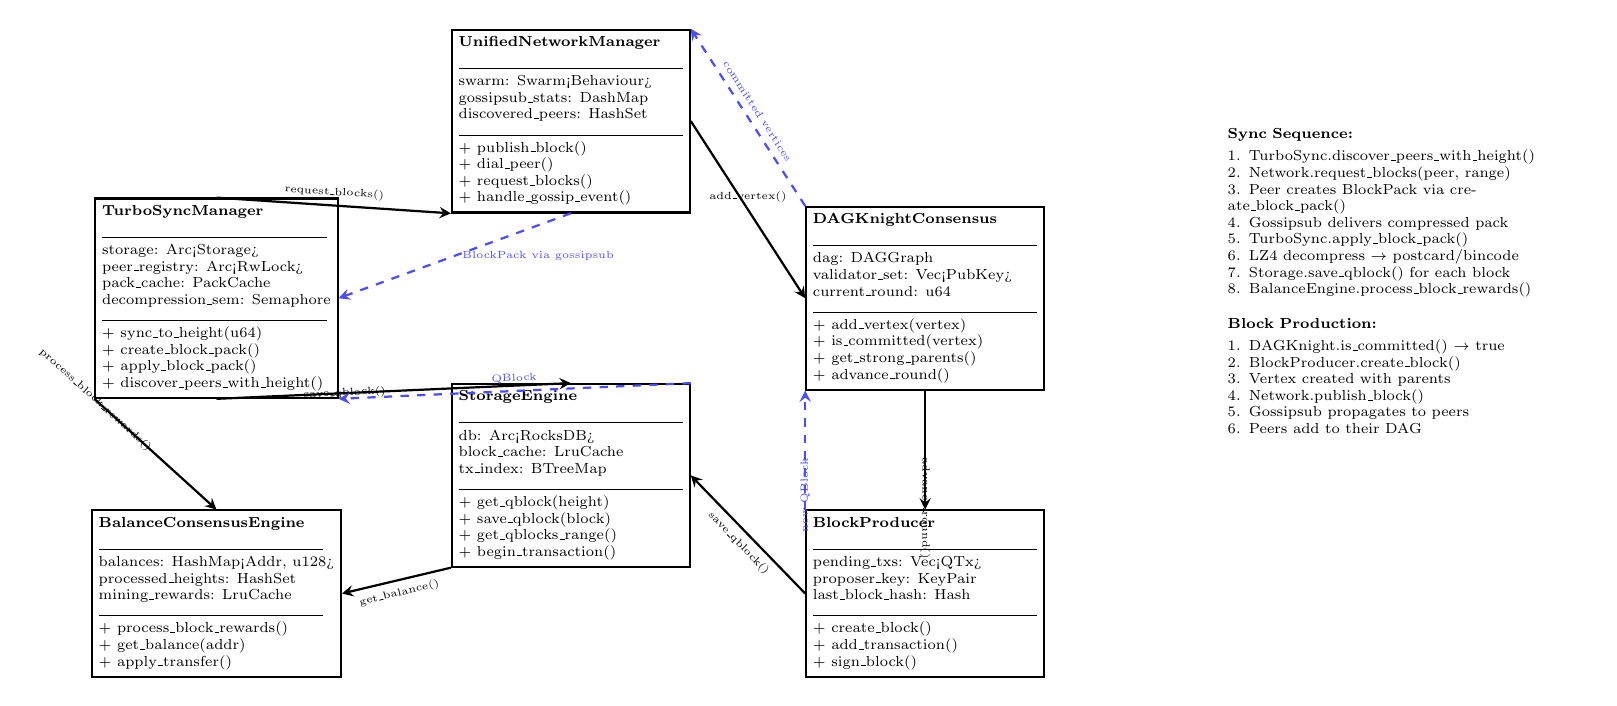
\begin{tikzpicture}[
    scale=0.75,
    transform shape,
    class/.style={rectangle, draw=black, thick, fill=white, minimum width=4cm, minimum height=2.5cm, font=\scriptsize, align=left},
    method/.style={font=\tiny\ttfamily},
    arrow/.style={->, thick, >=stealth},
    msgarrow/.style={->, thick, >=stealth, dashed, blue!70}
]

% ========================================
% TurboSyncManager (Main Sync Class)
% ========================================
\node[class] (turbosync) at (0,0) {
    \textbf{TurboSyncManager}\\[0.1cm]
    \rule{3.8cm}{0.5pt}\\
    storage: Arc<Storage>\\
    peer\_registry: Arc<RwLock>\\
    pack\_cache: PackCache\\
    decompression\_sem: Semaphore\\
    \rule{3.8cm}{0.5pt}\\
    \method{+ sync\_to\_height(u64)}\\
    \method{+ create\_block\_pack()}\\
    \method{+ apply\_block\_pack()}\\
    \method{+ discover\_peers\_with\_height()}
};

% ========================================
% UnifiedNetworkManager
% ========================================
\node[class] (network) at (6,3) {
    \textbf{UnifiedNetworkManager}\\[0.1cm]
    \rule{3.8cm}{0.5pt}\\
    swarm: Swarm<Behaviour>\\
    gossipsub\_stats: DashMap\\
    discovered\_peers: HashSet\\
    \rule{3.8cm}{0.5pt}\\
    \method{+ publish\_block()}\\
    \method{+ dial\_peer()}\\
    \method{+ request\_blocks()}\\
    \method{+ handle\_gossip\_event()}
};

% ========================================
% StorageEngine
% ========================================
\node[class] (storage) at (6,-3) {
    \textbf{StorageEngine}\\[0.1cm]
    \rule{3.8cm}{0.5pt}\\
    db: Arc<RocksDB>\\
    block\_cache: LruCache\\
    tx\_index: BTreeMap\\
    \rule{3.8cm}{0.5pt}\\
    \method{+ get\_qblock(height)}\\
    \method{+ save\_qblock(block)}\\
    \method{+ get\_qblocks\_range()}\\
    \method{+ begin\_transaction()}
};

% ========================================
% DAGKnightConsensus
% ========================================
\node[class] (dagknight) at (12,0) {
    \textbf{DAGKnightConsensus}\\[0.1cm]
    \rule{3.8cm}{0.5pt}\\
    dag: DAGGraph\\
    validator\_set: Vec<PubKey>\\
    current\_round: u64\\
    \rule{3.8cm}{0.5pt}\\
    \method{+ add\_vertex(vertex)}\\
    \method{+ is\_committed(vertex)}\\
    \method{+ get\_strong\_parents()}\\
    \method{+ advance\_round()}
};

% ========================================
% BalanceConsensusEngine
% ========================================
\node[class] (balance) at (0,-5) {
    \textbf{BalanceConsensusEngine}\\[0.1cm]
    \rule{3.8cm}{0.5pt}\\
    balances: HashMap<Addr, u128>\\
    processed\_heights: HashSet\\
    mining\_rewards: LruCache\\
    \rule{3.8cm}{0.5pt}\\
    \method{+ process\_block\_rewards()}\\
    \method{+ get\_balance(addr)}\\
    \method{+ apply\_transfer()}
};

% ========================================
% BlockProducer
% ========================================
\node[class] (producer) at (12,-5) {
    \textbf{BlockProducer}\\[0.1cm]
    \rule{3.8cm}{0.5pt}\\
    pending\_txs: Vec<QTx>\\
    proposer\_key: KeyPair\\
    last\_block\_hash: Hash\\
    \rule{3.8cm}{0.5pt}\\
    \method{+ create\_block()}\\
    \method{+ add\_transaction()}\\
    \method{+ sign\_block()}
};

% ========================================
% Arrows with method calls
% ========================================

% TurboSync -> Network
\draw[arrow] (turbosync.north) -- node[above, font=\tiny, sloped] {request\_blocks()} (network.south west);
\draw[msgarrow] (network.south) -- node[right, font=\tiny] {BlockPack via gossipsub} (turbosync.east);

% TurboSync -> Storage
\draw[arrow] (turbosync.south) -- node[left, font=\tiny, sloped] {save\_qblock()} (storage.north);
\draw[msgarrow] (storage.north east) -- node[above, font=\tiny, sloped] {QBlock} (turbosync.south east);

% TurboSync -> Balance
\draw[arrow] (turbosync.south west) -- node[left, font=\tiny, sloped] {process\_block\_rewards()} (balance.north);

% Network -> DAGKnight
\draw[arrow] (network.east) -- node[above, font=\tiny] {add\_vertex()} (dagknight.west);
\draw[msgarrow] (dagknight.north west) -- node[above, font=\tiny, sloped] {committed vertices} (network.north east);

% DAGKnight -> Producer
\draw[arrow] (dagknight.south) -- node[right, font=\tiny, sloped] {advance\_round()} (producer.north);
\draw[msgarrow] (producer.north west) -- node[left, font=\tiny, sloped] {new QBlock} (dagknight.south west);

% Storage -> Balance
\draw[arrow] (storage.south west) -- node[below, font=\tiny, sloped] {get\_balance()} (balance.east);

% Producer -> Storage
\draw[arrow] (producer.west) -- node[below, font=\tiny, sloped] {save\_qblock()} (storage.east);

% ========================================
% Message Flow Sequence
% ========================================
\node[anchor=north west, text width=6cm, font=\scriptsize] at (17,3) {
    \textbf{Sync Sequence:}\\[0.1cm]
    1. TurboSync.discover\_peers\_with\_height()\\
    2. Network.request\_blocks(peer, range)\\
    3. Peer creates BlockPack via create\_block\_pack()\\
    4. Gossipsub delivers compressed pack\\
    5. TurboSync.apply\_block\_pack()\\
    6. LZ4 decompress $\rightarrow$ postcard/bincode\\
    7. Storage.save\_qblock() for each block\\
    8. BalanceEngine.process\_block\_rewards()\\[0.3cm]

    \textbf{Block Production:}\\[0.1cm]
    1. DAGKnight.is\_committed() $\rightarrow$ true\\
    2. BlockProducer.create\_block()\\
    3. Vertex created with parents\\
    4. Network.publish\_block()\\
    5. Gossipsub propagates to peers\\
    6. Peers add to their DAG
};

\end{tikzpicture}
\end{center}

% Third page: Decentralization Evidence
\newpage

\begin{center}
{\LARGE \textbf{Decentralization Architecture Evidence}}\\[0.3cm]
{\large Code-Level Analysis}\\[0.5cm]
\end{center}

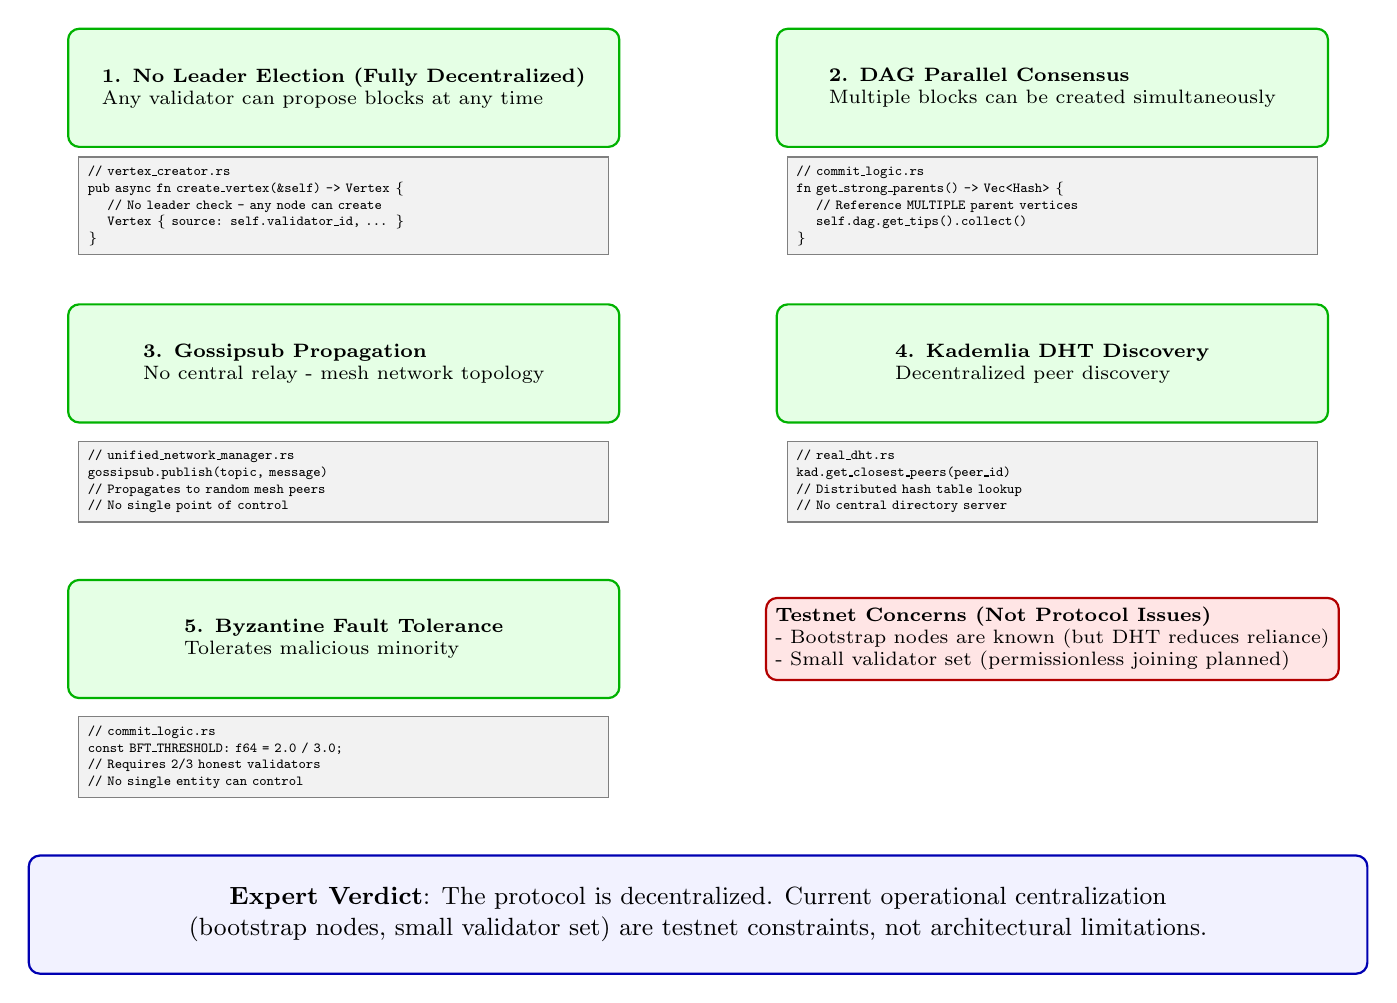
\begin{tikzpicture}[
    evidence/.style={rectangle, draw=green!70!black, thick, fill=green!10, rounded corners, minimum width=7cm, minimum height=1.5cm, font=\scriptsize, align=left},
    concern/.style={rectangle, draw=red!70!black, thick, fill=red!10, rounded corners, minimum width=7cm, minimum height=1cm, font=\scriptsize, align=left},
    code/.style={rectangle, draw=gray, fill=gray!10, font=\tiny\ttfamily, align=left, text width=6.5cm}
]

% Evidence 1: No Leader Election
\node[evidence] (e1) at (0,8) {
    \textbf{1. No Leader Election (Fully Decentralized)}\\
    Any validator can propose blocks at any time
};
\node[code] at (0,6.5) {
    // vertex\_creator.rs\\
    pub async fn create\_vertex(\&self) -> Vertex \{\\
    \ \ \ \ // No leader check - any node can create\\
    \ \ \ \ Vertex \{ source: self.validator\_id, ... \}\\
    \}
};

% Evidence 2: DAG Parallel Consensus
\node[evidence] (e2) at (9,8) {
    \textbf{2. DAG Parallel Consensus}\\
    Multiple blocks can be created simultaneously
};
\node[code] at (9,6.5) {
    // commit\_logic.rs\\
    fn get\_strong\_parents() -> Vec<Hash> \{\\
    \ \ \ \ // Reference MULTIPLE parent vertices\\
    \ \ \ \ self.dag.get\_tips().collect()\\
    \}
};

% Evidence 3: P2P Gossip
\node[evidence] (e3) at (0,4.5) {
    \textbf{3. Gossipsub Propagation}\\
    No central relay - mesh network topology
};
\node[code] at (0,3) {
    // unified\_network\_manager.rs\\
    gossipsub.publish(topic, message)\\
    // Propagates to random mesh peers\\
    // No single point of control
};

% Evidence 4: Kademlia DHT
\node[evidence] (e4) at (9,4.5) {
    \textbf{4. Kademlia DHT Discovery}\\
    Decentralized peer discovery
};
\node[code] at (9,3) {
    // real\_dht.rs\\
    kad.get\_closest\_peers(peer\_id)\\
    // Distributed hash table lookup\\
    // No central directory server
};

% Evidence 5: BFT Threshold
\node[evidence] (e5) at (0,1) {
    \textbf{5. Byzantine Fault Tolerance}\\
    Tolerates malicious minority
};
\node[code] at (0,-0.5) {
    // commit\_logic.rs\\
    const BFT\_THRESHOLD: f64 = 2.0 / 3.0;\\
    // Requires 2/3 honest validators\\
    // No single entity can control
};

% Concerns
\node[concern] (c1) at (9,1) {
    \textbf{Testnet Concerns (Not Protocol Issues)}\\
    - Bootstrap nodes are known (but DHT reduces reliance)\\
    - Small validator set (permissionless joining planned)
};

% Summary box
\node[rectangle, draw=blue!70!black, thick, fill=blue!5, rounded corners, minimum width=17cm, minimum height=1.5cm, font=\small, align=center] at (4.5,-2.5) {
    \textbf{Expert Verdict}: The protocol is decentralized. Current operational centralization\\
    (bootstrap nodes, small validator set) are testnet constraints, not architectural limitations.
};

\end{tikzpicture}

\vfill
\begin{center}
\rule{15cm}{0.5pt}\\[0.2cm]
{\small Q-NarwhalKnight v2.1.x-DELTA-V Architecture Document}\\
{\tiny Generated December 2024}
\end{center}

\end{document}
